\documentclass[12pt,a4paper,oneside]{report}             % Single-side
%\documentclass[12pt,a4paper,twoside,openright]{report}  % Duplex

%\PassOptionsToPackage{chapternumber=Huordinal}{magyar.ldf}
\usepackage{bm}
\usepackage{amsmath}
\usepackage{amssymb}
\usepackage{enumerate}
\usepackage[thmmarks]{ntheorem}
\usepackage{graphics}
\usepackage{epsfig}
\usepackage{listings}
\usepackage{color}
\usepackage{algorithm}
\usepackage{algorithmic}
\usepackage{lastpage}
\usepackage{anysize}
\usepackage{sectsty}
\usepackage{setspace}  % Ettol a tablazatok, abrak, labjegyzetek maradnak 1-es sorkozzel!
\usepackage[hang]{caption}
\usepackage{hyperref}
\usepackage[magyar]{babel}
\usepackage{fontspec}
\usepackage{textcomp}
\usepackage{subcaption}
\usepackage{titlesec, blindtext, color}
\usepackage{fancyhdr}
\usepackage{lastpage}
\usepackage{todonotes}
\usepackage{graphicx}
\usepackage{tikz}
\usepackage{subcaption}
\usepackage{float}
\usepackage{listings}
\usepackage{xcolor}
\usepackage[sorting=none, backend=biber, style=ieee]{biblatex}
\usepackage{courier}
\addbibresource{bib.bib}
\lstloadaspects{formats}

\definecolor{commentgreen}{RGB}{0,200,10}
\definecolor{weborange}{RGB}{255,10,0}
\definecolor{frenchplum}{RGB}{129,20,83}
\definecolor{codegray}{rgb}{0.5,0.5,0.5}
\definecolor{backcolour}{rgb}{0.95,0.95,0.92}

\setlength{\headheight}{14.5pt}

\lstdefinestyle{mystyle}{
	backgroundcolor=\color{backcolour},   
	commentstyle=\color{codegray},
	keywordstyle=\bf\color{frenchplum},
	numberstyle=\color{frenchplum},
	stringstyle=\color{commentgreen},
	basicstyle=\ttfamily\footnotesize,
	breakatwhitespace=false, 
	fontadjust=true,        
	breaklines=true,                 
	captionpos=b,
	columns=flexible,                   
	keepspaces=true,                 
	numbers=none,                    
	numbersep=5pt,                  
	showspaces=false,                
	showstringspaces=false,
	showtabs=false,                 
	tabsize=4
}

\lstset{style=mystyle}

%--------------------------------------------------------------------------------------
% Main variables
%--------------------------------------------------------------------------------------
\newcommand{\vikauthor}{Szemenyei Márton, Reizinger Patrik}
\newcommand{\viktitle}{M7 – Objektumkövetés mélység kamera segítségével}
\newcommand{\vikdept}{Irányítástechnika és Informatika Tanszék}
\newcommand{\vikdoktipus}{Irányítástechnika és Képfeldolgozás Laboratórium 1.}
\newcommand{\viksubtitle}{Mérési Útmutató}

%--------------------------------------------------------------------------------------
% Page layout setup
%--------------------------------------------------------------------------------------
% we need to redefine the pagestyle plain
% another possibility is to use the body of this command without \fancypagestyle
% and use \pagestyle{fancy} but in that case the special pages
% (like the ToC, the References, and the Chapter pages)remain in plane style

\pagestyle{plain}
\setlength{\parindent}{0pt} % �ttekinthet�bb, angol nyelv� dokumentumokban jellemz�
\setlength{\parskip}{8pt plus 3pt minus 3pt} % �ttekinthet�bb, angol nyelv� dokumentumokban jellemz�
%\setlength{\parindent}{12pt} % magyar nyelv� dokumentumokban jellemz�
%\setlength{\parskip}{0pt}    % magyar nyelv� dokumentumokban jellemz�

\marginsize{35mm}{25mm}{15mm}{15mm} % anysize package
\setcounter{secnumdepth}{0}
\sectionfont{\large\upshape\bfseries}
\setcounter{secnumdepth}{2}

%--------------------------------------------------------------------------------------
%	Setup hyperref package
%--------------------------------------------------------------------------------------
\hypersetup{
    pdftitle={\viktitle},        % title
    pdfauthor={\vikauthor},    % author
    pdfsubject={\vikdoktipus}, % subject of the document
    pdfcreator={\vikauthor},   % creator of the document
    pdfkeywords={Számítógépes látás, Objektumkövetés, RGBD},    % list of keywords
    pdfnewwindow=true,         % links in new window
    colorlinks=true,           % false: boxed links; true: colored links
    linkcolor=black,           % color of internal links
    citecolor=black,           % color of links to bibliography
    filecolor=black,           % color of file links
    urlcolor=black             % color of external links
}	

%--------------------------------------------------------------------------------------
%	Some new commands and declarations
%--------------------------------------------------------------------------------------
\newcommand{\code}[1]{{\upshape\ttfamily\scriptsize\indent #1}}

% define references
\newcommand{\figref}[1]{\ref{fig:#1}.}
\renewcommand{\eqref}[1]{(\ref{eq:#1})}
\newcommand{\listref}[1]{\ref{listing:#1}.}
\newcommand{\sectref}[1]{\ref{sect:#1}}
\newcommand{\tabref}[1]{\ref{tab:#1}.}

\DeclareMathOperator*{\argmax}{arg\,max}
%\DeclareMathOperator*[1]{\floor}{arg\,max}
\DeclareMathOperator{\sign}{sgn}
\DeclareMathOperator{\rot}{rot}
\definecolor{lightgray}{rgb}{0.95,0.95,0.95}

\newcommand{\hsp}{\hspace{20pt}}
\titlespacing*{\chapter}{0pt}{0pt}{40pt}


\author{\vikauthor}
\title{\viktitle}
%--------------------------------------------------------------------------------------
%	Setup captions
%--------------------------------------------------------------------------------------
\captionsetup[figure]{
%labelsep=none,
%font={footnotesize,it},
%justification=justified,
width=.9\textwidth,
aboveskip=10pt}

\renewcommand{\captionlabelfont}{\small\bf}
\renewcommand{\captionfont}{\footnotesize\it}

\fancypagestyle{plain}{%
	\fancyhf{}
	\renewcommand{\footrulewidth}{1pt}
	\chead{\viktitle}
	\lfoot{\thepage/\pageref{LastPage}} %/\pagetotal
	\rfoot{\leftmark}
}
\pagestyle{plain}

\pagestyle{fancy}
\fancyhf{}
\chead{\viktitle}
\lfoot{\thepage/\pageref{LastPage}} %/\pagetotal
\rfoot{\leftmark}
\renewcommand{\footrulewidth}{1pt}

%--------------------------------------------------------------------------------------
% Table of contents and the main text
%--------------------------------------------------------------------------------------
\begin{document}

\onehalfspacing

%--------------------------------------------------------------------------------------
%	The title page
%--------------------------------------------------------------------------------------
\begin{titlepage}
\begin{center}

\includegraphics[width=60mm,keepaspectratio]{images/logo.png}\\
\vspace{0.3cm}
\textbf{Budapesti Műszaki és Gazdaságtudományi Egyetem}\\
\textmd{Villamosmérnöki és Informatikai Kar}\\
\textmd{\vikdept}\\[5cm]

\vspace{0.4cm}
{\huge \bfseries \viktitle}\\[2cm]
\textsc{\Large \viksubtitle}\\[1cm]
\textsc{\Large \vikdoktipus}\\[6cm]

\vfill
{\large \vikauthor}
\end{center}
\end{titlepage}

%\pagenumbering{arabic}

%--------------------------------------------------------------------------------------
% tartalom, ábra és táblázatjegyzék
%--------------------------------------------------------------------------------------
\singlespacing
\tableofcontents\thispagestyle{fancy}
\titleformat{\chapter}[hang]{\Huge\bfseries}{\thechapter\hsp}{0pt}{\Huge\bfseries}
\onehalfspacing

\chapter{Objektumfelismerés}

A kamerarendszerek egyik legfontosabb felhasználási célja a környezetben található objektumok szétválasztása és a lényeges elemek kiemelése, más szóval szegmentálás. Tekintettel a fontosságára, illetve a feladat meglehetősen nem egzakt jellegére, számos jó és kevésbé jó algoritmust alkalmazhatunk. Legtöbbjük csak különleges körülmények között használható, vagy olyan mértékű futásidőigénye, hogy a legtöbb alkalmazásban szóba se kerülhet. Emiatt az alkalmazások nagy részénél valamilyen módon egyszerűsítenünk kell a környezetet, és olyan módon kell átalakítanunk, hogy az algoritmus számára könnyedén feldolgozható legyen. Erre megoldás, ha a megkeresendő objektum színét megváltoztatjuk olyan módon, hogy a környezettől elüssön.

A szegmentált objektumok megtalálása után annak releváns tulajdonságait is meg kell határoznunk. Szinte minden esetben szükséges a pozíció és/vagy orientáció, de gyakran van szükség méretre stb. A lényeges tulajdonságok kiemelése általában egyszerűbb feladat, mint a szegmentálás, de sokszor ezek meghatározása is szinte lehetetlennek tűnik. Az alábbiakban ismertetünk néhány fontosabb algoritmust, amely segítségével a mérésben szükséges képfeldolgozási feladatok elvégezhetők. Ez természetesen nem jelenti, hogy a hallgató nem használhat szofisztikáltabb megoldást.

\section{RGB-D kamerák}

Az elmúlt néhány évben egyre inkább elterjedtek olyan speciális szenzorok, amelyek az egyes pixelek intenzitásai mellett azok a szenzortól számított távolságukat is képesek meghatározni, így minden egyes képponthoz egy negyedik számértéket is hozzárendelnek. Ezeket az eszközöket RGB-D, vagy mélység kameráknak nevezzük, ahol a D az angol depth, vagyis mélység szóból származik.

Ezeknek a kameráknak alapvetően két változata létezik: az elsőt sztereó kamerának nevezzük, ahol két, egymástól fix távolságra lévő kamera van egy házba építve, és az egyes pixelek távolságát és a két készített kép közötti megfeleltetésekből számolhatjuk ki. Ezeknek az eszközöknek a kalibrációja általában a gyártás során megtörténik, valamint a mélység számítása a kamerába épített feldolgozó hardveren megtörténik.

Ezzel szemben az infravörös technológiára alapuló mélység kamerák három elemből állnak: egy közönséges RBG érzékelőből, egy infravörös vetítőből és egy az infravörös tartományban működő érzékelőből. A működésük elve, hogy az ember számára láthatatlan infravörös tartományban egy előre meghatározott mintázatot vetítenek ki, amelyet az infravörös érzékelő visszaolvas, és a mintázat torzulásából következtet a látott kép térbeli struktúrájára. A kettő közül az infravörös alapú érzékelők elterjedtebbek, mivel jobb minőségű eredményeket adnak és kevesebb feldolgozást igényelnek. Hátrányuk, hogy a környezetben található egyéb infravörös források megzavarhatják az eredményeket.

\begin{figure}
	\centering
	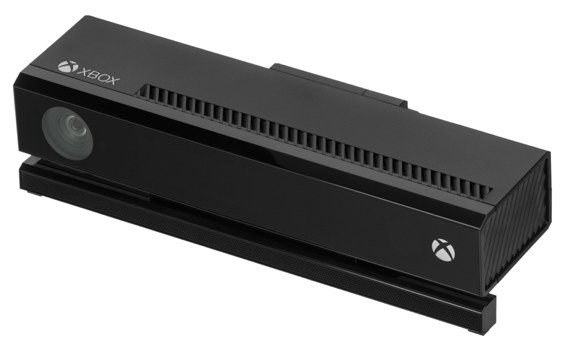
\includegraphics[width=0.75\textwidth]{images/Kinect.png}
	\label{fig:1}
	\caption{A Kinect One RGB-D érzékelő}
\end{figure}

Az RGB-D kamerák által szolgáltatott mélység kép (amely önmagában egy egyszerű szürkeárnyalatos kép) felhasználható arra, hogy a térben egybetartozó objektumokat könnyedén a kamerától valós távolság alapján szegmentálhassunk. Természetesen egymáshoz térben közel lévő objektumok a mélység képen „összenőhetnek”, így önmagában ez a módszer nem teljes mértékben megbízható.

\section{Szín alapú detektálás}

A számítógépes látás~\cite{szgl} során gyakran használjuk ki a szürkeárnyalatos képekben rejlő intenzitás információn felül a színes képek által hordozott extra információt is. Számos egyszerű detektáló algoritmus épül színbeli hasonlóság alapú keresésre. Itt azonban számos problémába ütközhetünk: egyrészt ahhoz, hogy a színbeli hasonlóság alapú keresés megbízhatóan, robusztusan működjön, arra van szükség, hogy a színeket leíró pixel értékek segítségével könnyen ki tudjuk fejezni a színek hasonlóságát. 

A kamerák által leggyakrabban használt színábrázolás (vagy más néven az RGB színtér) azonban erre nem alkalmas: két színt leíró pont geometriai távolsága az RGB színtérben nem kifejező arra nézve, hogy az emberi érzékelés mennyire érzi hasonlónak a két színt. Ezen felül amennyiben a megvilágítási viszonyok megváltoznak, az egy RGB kép esetén mind a három értéket megváltoztatja, pedig a képen található objektum színe nem változott.

A színtér transzformációs eljárások célja, hogy az RGB helyett egy olyan új színreprezentációt adjanak meg, amely információ elveszítése nélkül képes a színbeli hasonlóságot jól leírni, ezen felül pedig a megvilágítás változására is robusztus. Ezek a transzformációk ezzel egyben egy új színteret is definiálnak. A két leggyakrabban használt színtér az YCbCr család, illetve a HS\{V/I/L\} család. Ezekről a színterekről a Számítógépes Látórendszerek c. tárgy jegyzetében~\cite{szgl} olvashat bővebben.

\chapter{A mérés környezete}

A mérés során a \emph{PyCharm} elnevezésű IDE áll rendelkezésre, amely rendkívül sokoldalú szolgáltatásokkal könnyíti meg a szoftverfejlesztést, például konfigurálható automatikus formázási lehetőségek állnak rendelkezésünkre. További részletekért érdemes lehet a JetBrains ide vonatkozó weboldalát~\cite{pycharm} felkeresni. Függvények, objektumok esetében a \textbf{\textit{Ctrl+P}} billentyűkombináció pop-up segítségként szolgálva mutatja nekünk a paramétereket. A mérés során használt programnyelv a Python 3-as verziója lesz.

\section{A Python nyelv}

A Python programnyelv egy \textbf{\textit{interpretált szkriptnyelv}} (a saját bytekódját hajtja végre), mely alapvetően az \emph{objektumorientált} paradigma által vezérelve került kialakításra. Jelenleg kétféle, kismértékben eltérő főverziója érhető el, ezek közül a mérésen a 3-as verziót használjuk majd.

Az OOP szemlélet olyannyira központi szerepet tölt be Pythonban, hogy minden változó objektumnak tekinthető – ami azt jelenti, hogy az integer és float típusok is objektumok. A nyelv számára jelentős hátrány adatintenzív számítási feladatok elvégzésekor ennek ténye, ugyanis arról beszélünk, hogy a Python \textbf{\textit{nem rendelkezik natív számtípussal}}. Nem véletlen, hogy a hatékony modulok alacsonyabb szintű nyelveken nyugszanak, így a következő alfejezetben ismertetett PyTorch is.

További nem szokványos jellemzője a nyelvnek, hogy \textbf{\textit{nem erősen típusos}}, a változónevekhez futási időben rendelődik hozzá a referált objektum (azaz egy \textbf{\textit{változónév}} igazából egy referens, vagyis adott \textbf{\textit{példányra mutató referenciát}} tartalmaz). Habár Pythonban a referenciák teljesen úgy viselkednek, mint a változók (vagyis semmilyen szintaktikai kiegészítésre nincs szükség, még argumentumok átadása esetében sem, mint ahogy azt C++-ban láttuk). (A félreértések elkerülése végett fontos szem előtt tartani, hogy amennyiben a segédletben a továbbiakban változó szerepel, akkor is igazából referencia van a háttérben, ezért hangsúlyozott általában, hogy nem a változó, hanem a változónév tartalmazza az objektumra mutató referenciát.)

Vagyis lehetőség van arra, hogy egy referenshez (változónévhez) a programban különböző típusú objektumokat rendeljünk hozzá – ez teljesen logikusnak tűnik, ha belegondolunk abba, hogy a „Pythonban minden objektum” korábbi kijelentés lényegében azt sejteti, hogy minden az objektum ősosztály leszármazottja. A referenciák kezelése referenciaszámláló segítségével történik – a koncepció analóg a például C++-ban megtalálható \emph{shared\_ptr} típus esetén használttal.

Pythonban nincsen továbbá pointer sem, az argumentumok átadása \textbf{\textit{referencia szerint}} történik. Itt azonban meg kell különböztetnünk az objektumokat az alapján, hogy módosíthatóak-e. A következőket érdemes alaposan átgondolni, különben hibás működésű programot kaphatunk.

Kétféle objektumtípus létezik, \textbf{\textit{módosítható}} (mutable), ill. \textbf{\textit{nem módosítható}} (immutable). Nem módosíthatóak többek között az egyszerű adattípusok (POD, plain old data), mint az egész vagy lebegőpontos számok, valamint a sztringek. Habár a gondolatmenet e megfontolás mögött elsőre furcsának tűnik, a következőképpen magyarázható: minden adott szám vagy szöveg egyedi, vagyis ha pl. két változóhoz hozzárendeljük az 5 értéket, akkor a kettő tartalma egymással teljesen azonos, ha az egyiket megváltoztatjuk, akkor az már egy másik objektum lesz: nem egy tagváltozót módosítunk, hanem magát az objektumot teljes mértékben és kizárólagosan azonosító elemet. Talán érdemes a fordított programnyelvekből egy szemléletes példát átgondolni: a fordító ugyanolyan értékeket helyettesít be a gépi kódba (érdeklődők számára: a Pythonnak esetében is elérhető egyfajta disassembly a dis modul segítségével).

Módosítható lényegében minden egyéb típus, így a Pythonba beépített konténer jellegű típusok, mint list, dict (ezek különlegessége, hogy nem csak egy típust képesek egyidejűleg magukba foglalni, hanem bármilyen objektumot), de a saját osztályok példányai is ide tartoznak. Ebben az esetben a módosítás nem eredményezi új objektum létrehozását. A tuple egy különleges eset, ugyanis ez a konténer típus immutable, azonban, ha mutable objektumokat tartalmaz, akkor azok módosulhatnak.

Ezek a különbségek objektumok másolása esetében is jelentkezik. Fontos különbség, hogy Pythonban alapvetően a hozzárendelés (assignment) igazából C++-szemszögből inkább a copy constructor hívásának feleltethető meg. Immutable esetben az eredeti objektumhoz tartozó referenciszámláló kerül megnövelésre, módosítás esetén pedig új objektum jön létre, értelemszerűen ugyanazt az értéket tartalmazó változók egyikének megváltoztatása nem hat ki a többire. Mutable esetben azonban nem ilyen egyszerű a helyzet: mivel alapvetően referenciákat tartalmaznak a változónevek, amelyek módosítható objektumokat referálnak, így ugyanarra a példányra mutató referenciák bármelyikének módosítása változást eredményez a referált egy darab objektum esetében, vagyis bármelyik változóval hivatkozunk rá, a változás mindegyik esetben látható lesz számunkra. Az ilyen jellegű másolást shallow copy-nak szokás nevezni, melynek párja a deepcopy (elérhető a copy modulban), ami Pythonban mutable esetben is új példányt hoz létre, így az új objektum független lesz a többitől.

Paraméterek átadása hozzárendeléssel történik, ez azonban nagy objektumok esetében sem okoz komolyabb problémát, ugyanis a referenciák kerülnek csak másolásra. Ez a láthatóságra a következőképpen van hatással: ha a paraméter immutable és a függvénytörzsben módosításra kerül, akkor lényegében a függvény scope-jában egy ideiglenes objektum kerül létrehozásra, a függvényből visszatérve a változó megtartja eredeti értékét. Mutable esetben, mivel a referencia kerül másolásra, az objektumok másolásánál láttuk, hogy az általuk referált objektumok módosítása érvényes, bármelyik referenciájával hivatkozunk is rá, így a függvény visszatérését követően az objektum már módosult értékével használható.
Rendkívül hasznos tulajdonság, hogy a Python gyakorlatilag bármennyi visszatérési értéket támogat.
A nyelvi koncepciók ismertetése után a következőkben a szintaktikai részletek kerülnek összefoglalásra.

Pythonban a programkód tagolása indentálással történik, vagyis a kódblokkokat egy tabulátorral beljebb kell kezdeni (ha valamilyen okból üres függvényt, ciklust, stb, kívánunk írni, akkor is kell egy indentált blokk, ezt egy sorban, a pass utasítással valósíthatjuk meg, ami nem hajt végre semmilyen műveletet).

Modulok betöltésére az import utasítással van lehetőségünk, mégpedig kétféle módon: importálhatjuk a teljes modult, ekkor a modul minden osztálya/függvénye a modul neve után írt „.” (pont) operátorral érhető el, ha from-ot használunk, lehetőségünk van csak egyes elemeket betölteni, ekkor a modul nevét nem kell az importált elem neve elé kiírni.

\begin{lstlisting}[language=Python]
import module
m = module.MyClass()

import module as md
m = md.MyClass()

from module import MyClass, my_func
m = myClass()
\end{lstlisting}

Függvények a következő módon hozhatók létre:

\begin{lstlisting}[language=Python]
def func(x):
	x += 1
	print("x = ", x)
\end{lstlisting}

A def kulcsszó után a függvény neve, majd a paraméterlista kerül megadásra, azt követően pedig az indentált függvénytörzs következik.

Osztályok esetében sem bonyolult a konstrukció:

\begin{lstlisting}[language=Python]
class my_class(object):
	def __init__(self):
		self.x = 5
\end{lstlisting}

Pythonban a konstruktort az \_\_init\_\_ (2-2 aláhúzással) rutin testesíti meg, mint látható, a tagfüggvények is majdnem teljesen megegyeznek az általános függvényekkel, azzal a különbséggel, hogy az első argumentum mindenképpen az adott példányra vonatkozik (mint ahogy a this C++-ban) – ezt konvenció szerint self-nek szoktuk nevezni.
Öröklés esetén nincs más teendőnk, mint az object osztály helyett megadni az általunk választott ősosztályt, majd a konstruktorban meghívni az ősosztály konstruktorát a super, általánosan az ősosztályra használható objektum segítségével.

\begin{lstlisting}[language=Python]
class base_class(object):
	def __init__(self):
		print("I am Groot")
\end{lstlisting}

\begin{lstlisting}[language=Python]
class inherited_class(base_class):
	def __init__(self):
		super().__init__()
		print("I am inherited")
\end{lstlisting}

Aki mélyebben érdeklődik a Python nyelv iránt, annak érdemes felkeresnie további példaprogramokat és kódrészleteket~\cite{gist}, valamint a TMIT SmartLab blogjának bejegyzéseit~\cite{smart1,smart2} (angolul). 

A Python programnyelvhez számos hasznos függvénykönyvtár tartozik, melyek a mérési feladatok megvalósítását nagymértékben megkönnyítik. A Python nyelv egyik rendkívül kényelmes funkciója a beépített package manager, amelynek segítségével az egyes könyvtárak automatikusan telepíthetők, telepítsük után pedig minden további beállítás nélkül használhatók. A Pythonhoz két ilyen package manager is tartozik, az egyik a Pip, amely a legtöbb telepíthető Python verzió mellé automatikusan települ, a másik pedig az Anaconda~\cite{conda}, ami a könyvtárkezelési funkciókon túl virtuális környezeteket is képes kezelni.

A Python egyik legfontosabb függvénykönyvtára a Numpy, amely tömbök kezelésére, illetve számtalan numerikus algoritmus használatára ad lehetőséget. A Numpy funkcionalitását kiegészíti a MatplotLib, melynek segítségével különböző ábrákat készíthetünk a tömbjeinkről. Egy harmadik rendkívül hasznos könyvtárcsalád a scikit, ami számos tudományos számításhoz szükséges alkönyvtárt foglal össze. A sckit-image képek kezelésére, a scikit-learn gépi tanulás algoritmusok használatára, míg a scikit-fuzzy fuzzy logika használatára ad lehetőséget. Ezek a könyvtárak tulajdonképpen együttesen kiadják a Matlab funkcionalitásának jelentős részét.

\section{OpenCV}

Az OpenCV~\cite{opencv} egy nyílt forráskódú számítógépes látás algoritmusokat tartalmazó függvénykönyvtár. Az OpenCV elsődleges nyelve a C++, azonban elérhetőek hozzá hivatalos wrapperek többek között Java és Python nyelven. Az OpenCV rengeteg hivatalosan támogatott algoritmust tartalmaz, melyen felül a külön letölthető Contrib modulban harmadik felek által kifejlesztett további funkciók is elérhetők.

\subsection{Adattípusok}

Az OpenCV könyvtár a Python verzióban a Numpy könyvtár által definiált n dimenziós számtömböket (ndarray) használja a képek tárolására. Ezek a tömbök különböző adattípusokat tartalmazhatnak, méretük minden kép esetén $H\times W\times c$, ahol $c$ a csatornák, $H$ a képsorok, $W$ pedig az oszlopok száma. Az egyszerűbb képi adattípusok egy azonosítóval is definiálhatóak az alábbi formában:

\begin{center} 
	CV\_<bitmélység>{U|S|F}C<csatornák száma>
\end{center} 

Bár tömbök segítségével közvetlenül is tárolhatnánk többdimenziós adatokat, a csatornák számának közvetlen megadása kényelmesebbé és szemléletesebbé teszi az adattárolást és programozást. Például színes képek esetén három csatornára van szükségünk, esetleg négyre, ha az időt is tárolni akarjuk.
Példák:
\begin{itemize}
	\item CV\_32F: 32 bites lebegőpontos szám
	\item CV\_8UC3: 8 bites 3 csatornás szám/kép
\end{itemize}

\subsection{Numpy tömbök manipulációja}

Üres $3\times 4$ tömb létrehozása:

\begin{lstlisting}[language=Python]
arr = np.ndarray((3,4))
\end{lstlisting}

Nullákkal/egyesekkel feltöltött $3\times 4$ tömb létrehozása:

\begin{lstlisting}[language=Python]
arr = np.zeros((3,4))
arr = np.ones((3,4))
\end{lstlisting}

Nullákkal/egyesekkel feltöltött, egy másik tömbbel megegyező méretű és típusú tömb létrehozása:

\begin{lstlisting}[language=Python]
arr1 = np.zeros_like(arr)
arr1 = np.ones_like(arr)
\end{lstlisting}

Lista-tömb konverzió:

\begin{lstlisting}[language=Python]
arr = np.array([[1,2,3],[4,5,6]])
\end{lstlisting}

Típuskonverzió:

\begin{lstlisting}[language=Python]
arr1 = arr.astype('float32')
arr1 = arr.astype('float64')
arr1 = arr.astype('uint8')
arr1 = arr.astype('int16')
\end{lstlisting}

Tömb mérete és adattípusa:

\begin{lstlisting}[language=Python]
arr.shape
arr.dtype
\end{lstlisting}

Tömb eleméhez történő hozzáférés:

\begin{lstlisting}[language=Python]
arr[2,2] # egy elem
arr[-1,-1] # utolsó sor utolsó eleme
arr[1:4,2:5] # részmátrix kiemelése (FONTOS: A felsö limit nem inkluzív, vagyis az [1-4) sor és a [2-5) oszlop vannak benne)
arr[1:3,:] # [1-3) sorok összes eleme 

rowInd = [1,3,5,11]
arr[rowInd] # Az 1,3,5 éa 11 sorok összes eleme

colBin = [True,True,False,True,False,False]
arr[:,colBin] # az összes sor 0,1 és 3 oszlopai
\end{lstlisting}

\subsection{Képek olvasása és megjelenítése}

Az első programunk egy keretprogram, melyet a mérés során folyamatosan módosítunk, bővítünk. A program rendkívül egyszerű, az OpenCV imread(), namedWindow() és imshow() függvényei megjelenítik egy ablakban a képet, majd az „ESC” gomb hatására program visszatér az operációs rendszerhez.

\begin{lstlisting}[language=Python]
import cv2
import numpy as np

img = cv2.imread("image.jpg",cv2.IMREAD_COLOR)
cv2.imshow("Image",img)
cv2.waitKey(0) # Waits for keyboard press - necessary after imshow
\end{lstlisting}

A cv2.IMREAD\_COLOR egy logikai változó (ún. flag), mely megmondja az imread függvénynek, hogy a képet színesként, három csatornán töltse be.  Alternatívaként, a cv2.IMREAD\_GRAYSCALE flag használatával lehetőség van a képet szürkeárnyalatosként, egyetlen csatornán betölteni. Fontos opció továbbá a cv2.IMREAD\_UNCHANGED melyet gyakran használunk RGB-D kamerák esetén a mélység kép betöltésére, mivel ezek általában egy csatornás, 16 bites képek, így a többi flag esetén elvégzett 8 bites konverzió adatvesztéshez vezetne.

A mérés során az eredmények mentéséhez és a mérési jegyzőkönyvhöz szükségünk lesz a képek kiírására, amihez az alábbi utasítás használható:

\begin{lstlisting}[language=Python]
cv2.imwrite("img_out.jpg",img)
\end{lstlisting}

\chapter{Mérési feladatok}

A mérés során a feladat egy a mérésvezető által meghatározott objektum térbeli követése lesz egy RGB-D szenzor segítségével. A mérés folyamán az alábbi feladatokat kell elvégezni:

\begin{enumerate}
\item Készítsen eljárást egy adott objektum 2D-ben történő követésére egy RGB-D kamera mélységképe alapján!
\item Készítsen eljárást egy adott objektum szín alapú követésére a HSV színtérben!
\item Határozza meg az adott objektum koordinátáit a 3D térben! Használjon Kalman-szűrőt (Kalman.py) az objektumok robusztus pozícióbecslésére!
\item Ellenőrizze az algoritmus helyes működését előre felvett videofelvételek, valamint élő videó segítségével!
\end{enumerate}

\chapter{Hasznos kódrészletek}

Részlet kivágása a képből

\begin{lstlisting}[language=Python]
array[y1:y2,x1:x2]
\end{lstlisting}

Középső depth érték kinyerése

\begin{lstlisting}[language=Python]
midDepth = int(depthRoi[self.height // 2, self.width // 2])
\end{lstlisting}

Küszöbözés adott tartományban

\begin{lstlisting}[language=Python]
roiMask = cv2.inRange(depthRoi, np.array([minval]), np.array([maxval]))
\end{lstlisting}

Egy másikkal egyező méretű csupa nulla kép készítése

\begin{lstlisting}[language=Python]
mask = np.zeros_like(binary)
\end{lstlisting}

Kontúrok keresése

\begin{lstlisting}[language=Python]
contours, _ = cv2.findContours(binary, cv2.RETR_EXTERNAL, cv2.CHAIN_APPROX_SIMPLE)
\end{lstlisting}

Maximum keresése

\begin{lstlisting}[language=Python]
maxidx = np.argmax([function(element) for element in list])
\end{lstlisting}

Kontúr területének számítása

\begin{lstlisting}[language=Python]
area = cv2.contourArea(cont)
\end{lstlisting}

Kontúr rajzolása:

\begin{lstlisting}[language=Python]
cv2.drawContours(mask, contours, maxInd, 255, -1)
\end{lstlisting}

Momentumok számítása

\begin{lstlisting}[language=Python]
moments = cv2.moments(contours[maxInd])
\end{lstlisting}

Tömegközéppont számítása

\begin{lstlisting}[language=Python]
self.cog = (int(moments['m10']/moments['m00']) + self.BB[2], int(moments['m01']/moments['m00']) + self.BB[0])
\end{lstlisting}

HSV konverzió

\begin{lstlisting}[language=Python]
imgHsv= cv2.cvtColor(imgRoi, cv2.COLOR_BGR2HSV)
\end{lstlisting}

Kép maszkolása

\begin{lstlisting}[language=Python]
maskedImgHsv = cv2.bitwise_and(image, image, mask=mask)
\end{lstlisting}

Csatornánkénti szétválasztás

\begin{lstlisting}[language=Python]
hueImg = maskedImgHsv[:, :, 0]
\end{lstlisting}

Bináris maszkok kombinálása

\begin{lstlisting}[language=Python]
hueMask = np.logical_and(cond1, cond2)
\end{lstlisting}

Bináris maszk alkalmazása

\begin{lstlisting}[language=Python]
hueVals = hueImg[hueMask]
\end{lstlisting}

Hisztogram számítása

\begin{lstlisting}[language=Python]
h = np.histogram(hueVals, 179)[0]
\end{lstlisting}

Maximum pozíció meghatározása

\begin{lstlisting}[language=Python]
np.argmax(h) 
\end{lstlisting}


\chapter{Ellenőrző kérdések}

\begin{enumerate}
\item Ismertesse röviden az RGB-D kamerák működési elvét!
\item Mi az a HSV színtér? Mire használhatjuk, és mi a használatának előnye?
\item Hogyan lehet egy bináris képen az objektumok kontúrjait meghatározni? Mire használhatók ezek fel?
\item Hogyan lehet egy bináris objektum tömegközéppontját meghatározni?
\item Milyen programozási nyelvet használunk a mérés során? Miért előnyös ez a nyelv multi-platform fejlesztés esetén?
\item Hogyan lehet osztályt és függvényt definiálni Python nyelven? (pszeudokód elég)
\end{enumerate}

\printbibliography

\end{document}

